% Options for packages loaded elsewhere
\PassOptionsToPackage{unicode}{hyperref}
\PassOptionsToPackage{hyphens}{url}
\PassOptionsToPackage{dvipsnames,svgnames,x11names}{xcolor}
%
\documentclass[
  letterpaper,
  DIV=11,
  numbers=noendperiod]{scrartcl}

\usepackage{amsmath,amssymb}
\usepackage{iftex}
\ifPDFTeX
  \usepackage[T1]{fontenc}
  \usepackage[utf8]{inputenc}
  \usepackage{textcomp} % provide euro and other symbols
\else % if luatex or xetex
  \usepackage{unicode-math}
  \defaultfontfeatures{Scale=MatchLowercase}
  \defaultfontfeatures[\rmfamily]{Ligatures=TeX,Scale=1}
\fi
\usepackage{lmodern}
\ifPDFTeX\else  
    % xetex/luatex font selection
\fi
% Use upquote if available, for straight quotes in verbatim environments
\IfFileExists{upquote.sty}{\usepackage{upquote}}{}
\IfFileExists{microtype.sty}{% use microtype if available
  \usepackage[]{microtype}
  \UseMicrotypeSet[protrusion]{basicmath} % disable protrusion for tt fonts
}{}
\makeatletter
\@ifundefined{KOMAClassName}{% if non-KOMA class
  \IfFileExists{parskip.sty}{%
    \usepackage{parskip}
  }{% else
    \setlength{\parindent}{0pt}
    \setlength{\parskip}{6pt plus 2pt minus 1pt}}
}{% if KOMA class
  \KOMAoptions{parskip=half}}
\makeatother
\usepackage{xcolor}
\setlength{\emergencystretch}{3em} % prevent overfull lines
\setcounter{secnumdepth}{5}
% Make \paragraph and \subparagraph free-standing
\makeatletter
\ifx\paragraph\undefined\else
  \let\oldparagraph\paragraph
  \renewcommand{\paragraph}{
    \@ifstar
      \xxxParagraphStar
      \xxxParagraphNoStar
  }
  \newcommand{\xxxParagraphStar}[1]{\oldparagraph*{#1}\mbox{}}
  \newcommand{\xxxParagraphNoStar}[1]{\oldparagraph{#1}\mbox{}}
\fi
\ifx\subparagraph\undefined\else
  \let\oldsubparagraph\subparagraph
  \renewcommand{\subparagraph}{
    \@ifstar
      \xxxSubParagraphStar
      \xxxSubParagraphNoStar
  }
  \newcommand{\xxxSubParagraphStar}[1]{\oldsubparagraph*{#1}\mbox{}}
  \newcommand{\xxxSubParagraphNoStar}[1]{\oldsubparagraph{#1}\mbox{}}
\fi
\makeatother

\usepackage{color}
\usepackage{fancyvrb}
\newcommand{\VerbBar}{|}
\newcommand{\VERB}{\Verb[commandchars=\\\{\}]}
\DefineVerbatimEnvironment{Highlighting}{Verbatim}{commandchars=\\\{\}}
% Add ',fontsize=\small' for more characters per line
\usepackage{framed}
\definecolor{shadecolor}{RGB}{241,243,245}
\newenvironment{Shaded}{\begin{snugshade}}{\end{snugshade}}
\newcommand{\AlertTok}[1]{\textcolor[rgb]{0.68,0.00,0.00}{#1}}
\newcommand{\AnnotationTok}[1]{\textcolor[rgb]{0.37,0.37,0.37}{#1}}
\newcommand{\AttributeTok}[1]{\textcolor[rgb]{0.40,0.45,0.13}{#1}}
\newcommand{\BaseNTok}[1]{\textcolor[rgb]{0.68,0.00,0.00}{#1}}
\newcommand{\BuiltInTok}[1]{\textcolor[rgb]{0.00,0.23,0.31}{#1}}
\newcommand{\CharTok}[1]{\textcolor[rgb]{0.13,0.47,0.30}{#1}}
\newcommand{\CommentTok}[1]{\textcolor[rgb]{0.37,0.37,0.37}{#1}}
\newcommand{\CommentVarTok}[1]{\textcolor[rgb]{0.37,0.37,0.37}{\textit{#1}}}
\newcommand{\ConstantTok}[1]{\textcolor[rgb]{0.56,0.35,0.01}{#1}}
\newcommand{\ControlFlowTok}[1]{\textcolor[rgb]{0.00,0.23,0.31}{\textbf{#1}}}
\newcommand{\DataTypeTok}[1]{\textcolor[rgb]{0.68,0.00,0.00}{#1}}
\newcommand{\DecValTok}[1]{\textcolor[rgb]{0.68,0.00,0.00}{#1}}
\newcommand{\DocumentationTok}[1]{\textcolor[rgb]{0.37,0.37,0.37}{\textit{#1}}}
\newcommand{\ErrorTok}[1]{\textcolor[rgb]{0.68,0.00,0.00}{#1}}
\newcommand{\ExtensionTok}[1]{\textcolor[rgb]{0.00,0.23,0.31}{#1}}
\newcommand{\FloatTok}[1]{\textcolor[rgb]{0.68,0.00,0.00}{#1}}
\newcommand{\FunctionTok}[1]{\textcolor[rgb]{0.28,0.35,0.67}{#1}}
\newcommand{\ImportTok}[1]{\textcolor[rgb]{0.00,0.46,0.62}{#1}}
\newcommand{\InformationTok}[1]{\textcolor[rgb]{0.37,0.37,0.37}{#1}}
\newcommand{\KeywordTok}[1]{\textcolor[rgb]{0.00,0.23,0.31}{\textbf{#1}}}
\newcommand{\NormalTok}[1]{\textcolor[rgb]{0.00,0.23,0.31}{#1}}
\newcommand{\OperatorTok}[1]{\textcolor[rgb]{0.37,0.37,0.37}{#1}}
\newcommand{\OtherTok}[1]{\textcolor[rgb]{0.00,0.23,0.31}{#1}}
\newcommand{\PreprocessorTok}[1]{\textcolor[rgb]{0.68,0.00,0.00}{#1}}
\newcommand{\RegionMarkerTok}[1]{\textcolor[rgb]{0.00,0.23,0.31}{#1}}
\newcommand{\SpecialCharTok}[1]{\textcolor[rgb]{0.37,0.37,0.37}{#1}}
\newcommand{\SpecialStringTok}[1]{\textcolor[rgb]{0.13,0.47,0.30}{#1}}
\newcommand{\StringTok}[1]{\textcolor[rgb]{0.13,0.47,0.30}{#1}}
\newcommand{\VariableTok}[1]{\textcolor[rgb]{0.07,0.07,0.07}{#1}}
\newcommand{\VerbatimStringTok}[1]{\textcolor[rgb]{0.13,0.47,0.30}{#1}}
\newcommand{\WarningTok}[1]{\textcolor[rgb]{0.37,0.37,0.37}{\textit{#1}}}

\providecommand{\tightlist}{%
  \setlength{\itemsep}{0pt}\setlength{\parskip}{0pt}}\usepackage{longtable,booktabs,array}
\usepackage{calc} % for calculating minipage widths
% Correct order of tables after \paragraph or \subparagraph
\usepackage{etoolbox}
\makeatletter
\patchcmd\longtable{\par}{\if@noskipsec\mbox{}\fi\par}{}{}
\makeatother
% Allow footnotes in longtable head/foot
\IfFileExists{footnotehyper.sty}{\usepackage{footnotehyper}}{\usepackage{footnote}}
\makesavenoteenv{longtable}
\usepackage{graphicx}
\makeatletter
\newsavebox\pandoc@box
\newcommand*\pandocbounded[1]{% scales image to fit in text height/width
  \sbox\pandoc@box{#1}%
  \Gscale@div\@tempa{\textheight}{\dimexpr\ht\pandoc@box+\dp\pandoc@box\relax}%
  \Gscale@div\@tempb{\linewidth}{\wd\pandoc@box}%
  \ifdim\@tempb\p@<\@tempa\p@\let\@tempa\@tempb\fi% select the smaller of both
  \ifdim\@tempa\p@<\p@\scalebox{\@tempa}{\usebox\pandoc@box}%
  \else\usebox{\pandoc@box}%
  \fi%
}
% Set default figure placement to htbp
\def\fps@figure{htbp}
\makeatother

% load packages
\usepackage{geometry}
\usepackage{xcolor}
\usepackage{eso-pic}
\usepackage{fancyhdr}
\usepackage{sectsty}
\usepackage{fontspec}
\usepackage{titlesec}

%% Set page size with a wider right margin
\geometry{a4paper, total={170mm,257mm}, left=20mm, top=20mm, bottom=20mm, right=50mm}

%% Let's define some colours
\definecolor{light}{HTML}{E6E6FA}
\definecolor{highlight}{HTML}{800080}
\definecolor{dark}{HTML}{330033}

%% Let's add the border on the right hand side 
\AddToShipoutPicture{% 
    \AtPageLowerLeft{% 
        \put(\LenToUnit{\dimexpr\paperwidth-3cm},0){% 
            \color{light}\rule{3cm}{\LenToUnit\paperheight}%
          }%
     }%
     % logo
    \AtPageLowerLeft{% start the bar at the bottom right of the page
        \put(\LenToUnit{\dimexpr\paperwidth-2.25cm},27.2cm){% move it to the top right
            \color{light}
\includegraphics[width=1.5cm]{_extensions/nrennie/PrettyPDF/logo.png}
          }%
     }%
}

%% Style the page number
\fancypagestyle{mystyle}{
  \fancyhf{}
  \renewcommand\headrulewidth{0pt}
  \fancyfoot[R]{\thepage}
  \fancyfootoffset{3.5cm}
}
\setlength{\footskip}{20pt}

%% style the chapter/section fonts
\chapterfont{\color{dark}\fontsize{20}{16.8}\selectfont}
\sectionfont{\color{dark}\fontsize{20}{16.8}\selectfont}
\subsectionfont{\color{dark}\fontsize{14}{16.8}\selectfont}
\titleformat{\subsection}
  {\sffamily\Large\bfseries}{\thesection}{1em}{}[{\titlerule[0.8pt]}]
  
% left align title
\makeatletter
\renewcommand{\maketitle}{\bgroup\setlength{\parindent}{0pt}
\begin{flushleft}
  {\sffamily\huge\textbf{\MakeUppercase{\@title}}} \vspace{0.3cm} \newline
  {\Large {\@subtitle}} \newline
  \@author
\end{flushleft}\egroup
}
\makeatother

%% Use some custom fonts
\setsansfont{Ubuntu}[
    Path=_extensions/nrennie/PrettyPDF/Ubuntu/,
    Scale=0.9,
    Extension = .ttf,
    UprightFont=*-Regular,
    BoldFont=*-Bold,
    ItalicFont=*-Italic,
    ]

\setmainfont{Ubuntu}[
    Path=_extensions/nrennie/PrettyPDF/Ubuntu/,
    Scale=0.9,
    Extension = .ttf,
    UprightFont=*-Regular,
    BoldFont=*-Bold,
    ItalicFont=*-Italic,
    ]
\usepackage{booktabs}
\usepackage{caption}
\usepackage{longtable}
\usepackage{colortbl}
\usepackage{array}
\usepackage{anyfontsize}
\usepackage{multirow}
\KOMAoption{captions}{tableheading}
\makeatletter
\@ifpackageloaded{tcolorbox}{}{\usepackage[skins,breakable]{tcolorbox}}
\@ifpackageloaded{fontawesome5}{}{\usepackage{fontawesome5}}
\definecolor{quarto-callout-color}{HTML}{909090}
\definecolor{quarto-callout-note-color}{HTML}{0758E5}
\definecolor{quarto-callout-important-color}{HTML}{CC1914}
\definecolor{quarto-callout-warning-color}{HTML}{EB9113}
\definecolor{quarto-callout-tip-color}{HTML}{00A047}
\definecolor{quarto-callout-caution-color}{HTML}{FC5300}
\definecolor{quarto-callout-color-frame}{HTML}{acacac}
\definecolor{quarto-callout-note-color-frame}{HTML}{4582ec}
\definecolor{quarto-callout-important-color-frame}{HTML}{d9534f}
\definecolor{quarto-callout-warning-color-frame}{HTML}{f0ad4e}
\definecolor{quarto-callout-tip-color-frame}{HTML}{02b875}
\definecolor{quarto-callout-caution-color-frame}{HTML}{fd7e14}
\makeatother
\makeatletter
\@ifpackageloaded{caption}{}{\usepackage{caption}}
\AtBeginDocument{%
\ifdefined\contentsname
  \renewcommand*\contentsname{Table of contents}
\else
  \newcommand\contentsname{Table of contents}
\fi
\ifdefined\listfigurename
  \renewcommand*\listfigurename{List of Figures}
\else
  \newcommand\listfigurename{List of Figures}
\fi
\ifdefined\listtablename
  \renewcommand*\listtablename{List of Tables}
\else
  \newcommand\listtablename{List of Tables}
\fi
\ifdefined\figurename
  \renewcommand*\figurename{Figure}
\else
  \newcommand\figurename{Figure}
\fi
\ifdefined\tablename
  \renewcommand*\tablename{Table}
\else
  \newcommand\tablename{Table}
\fi
}
\@ifpackageloaded{float}{}{\usepackage{float}}
\floatstyle{ruled}
\@ifundefined{c@chapter}{\newfloat{codelisting}{h}{lop}}{\newfloat{codelisting}{h}{lop}[chapter]}
\floatname{codelisting}{Listing}
\newcommand*\listoflistings{\listof{codelisting}{List of Listings}}
\makeatother
\makeatletter
\makeatother
\makeatletter
\@ifpackageloaded{caption}{}{\usepackage{caption}}
\@ifpackageloaded{subcaption}{}{\usepackage{subcaption}}
\makeatother
\makeatletter
\@ifpackageloaded{tcolorbox}{}{\usepackage[skins,breakable]{tcolorbox}}
\makeatother
\makeatletter
\@ifundefined{shadecolor}{\definecolor{shadecolor}{rgb}{.97, .97, .97}}{}
\makeatother
\makeatletter
\@ifundefined{codebgcolor}{\definecolor{codebgcolor}{named}{light}}{}
\makeatother
\makeatletter
\ifdefined\Shaded\renewenvironment{Shaded}{\begin{tcolorbox}[enhanced, frame hidden, breakable, colback={codebgcolor}, sharp corners, boxrule=0pt]}{\end{tcolorbox}}\fi
\makeatother

\usepackage{bookmark}

\IfFileExists{xurl.sty}{\usepackage{xurl}}{} % add URL line breaks if available
\urlstyle{same} % disable monospaced font for URLs
\hypersetup{
  pdftitle={Practical 6},
  colorlinks=true,
  linkcolor={highlight},
  filecolor={Maroon},
  citecolor={Blue},
  urlcolor={highlight},
  pdfcreator={LaTeX via pandoc}}


\title{Practical 6}
\author{}
\date{}

\begin{document}
\maketitle

\pagestyle{mystyle}


\textbf{Aim of this practical:}

In this practical we are going to look at some model comparison and
validation techniques.

\subsection{Model Checking for Linear
Models}\label{model-checking-for-linear-models}

In this exercise we will:

\begin{itemize}
\tightlist
\item
  Learn about some model assessments techniques available in INLA
\item
  Conduct posterior predictive model checking
\end{itemize}

Libraries to load:

\begin{Shaded}
\begin{Highlighting}[]
\FunctionTok{library}\NormalTok{(dplyr)}
\FunctionTok{library}\NormalTok{(tidyr)}
\FunctionTok{library}\NormalTok{(INLA)}
\FunctionTok{library}\NormalTok{(ggplot2)}
\FunctionTok{library}\NormalTok{(patchwork)}
\FunctionTok{library}\NormalTok{(inlabru)     }
\end{Highlighting}
\end{Shaded}

Recall a simple linear regression model with Gaussian observations

\[
y_i\sim\mathcal{N}(\mu_i, \sigma^2), \qquad i = 1,\dots,N
\]

where \(\sigma^2\) is the observation error, and the mean parameter
\(\mu_i\) is linked to the linear predictor through an identity
function:

\[
\eta_i = \mu_i = \beta_0 + \beta_1 x_i
\] where \(x_i\) is a covariate and \(\beta_0, \beta_1\) are parameters
to be estimated.

\subsubsection{Simulate example data}\label{simulate-example-data}

We simulate data from a simple linear regression model

\begin{Shaded}
\begin{Highlighting}[]
\NormalTok{beta }\OtherTok{=} \FunctionTok{c}\NormalTok{(}\DecValTok{2}\NormalTok{,}\FloatTok{0.5}\NormalTok{)}
\NormalTok{sd\_error }\OtherTok{=} \FloatTok{0.1}

\NormalTok{n }\OtherTok{=} \DecValTok{100}
\NormalTok{x }\OtherTok{=} \FunctionTok{rnorm}\NormalTok{(n)}
\NormalTok{y }\OtherTok{=}\NormalTok{ beta[}\DecValTok{1}\NormalTok{] }\SpecialCharTok{+}\NormalTok{ beta[}\DecValTok{2}\NormalTok{] }\SpecialCharTok{*}\NormalTok{ x }\SpecialCharTok{+} \FunctionTok{rnorm}\NormalTok{(n, }\AttributeTok{sd =}\NormalTok{ sd\_error)}

\NormalTok{df }\OtherTok{=} \FunctionTok{data.frame}\NormalTok{(}\AttributeTok{y =}\NormalTok{ y, }\AttributeTok{x =}\NormalTok{ x)  }
\end{Highlighting}
\end{Shaded}

\subsubsection{\texorpdfstring{Fitting the linear regression model with
\texttt{inlabru}}{Fitting the linear regression model with inlabru}}\label{fitting-the-linear-regression-model-with-inlabru}

Now we fit a simple linear regression model in \texttt{inalbru} by
defining (1) the model components, (2) the linear predictor and (3) the
likelihood.

\begin{Shaded}
\begin{Highlighting}[]
\CommentTok{\# Model components}
\NormalTok{cmp }\OtherTok{=}  \ErrorTok{\textasciitilde{}} \SpecialCharTok{{-}}\DecValTok{1} \SpecialCharTok{+} \FunctionTok{beta\_0}\NormalTok{(}\DecValTok{1}\NormalTok{) }\SpecialCharTok{+} \FunctionTok{beta\_1}\NormalTok{(x, }\AttributeTok{model =} \StringTok{"linear"}\NormalTok{)}
\CommentTok{\# Linear predictor}
\NormalTok{formula }\OtherTok{=}\NormalTok{ y }\SpecialCharTok{\textasciitilde{}}\NormalTok{ Intercept }\SpecialCharTok{+}\NormalTok{ beta\_1}
\CommentTok{\# Observational model likelihood}
\NormalTok{lik }\OtherTok{=}  \FunctionTok{bru\_obs}\NormalTok{(}\AttributeTok{formula =}\NormalTok{ y }\SpecialCharTok{\textasciitilde{}}\NormalTok{.,}
            \AttributeTok{family =} \StringTok{"gaussian"}\NormalTok{,}
            \AttributeTok{data =}\NormalTok{ df)}
\CommentTok{\# Fit the Model}
\NormalTok{fit.lm }\OtherTok{=} \FunctionTok{bru}\NormalTok{(cmp, lik)}
\end{Highlighting}
\end{Shaded}

\subsubsection{Residuals analysis}\label{residuals-analysis}

A common way for model diagnostics in regression analysis is by checking
residual plots. In a Bayesian setting residuals can be defined in
multiple ways depending on how you account for posterior uncertainty.
Here, we will adopt a Bayesian approach by generating samples from the
posterior distribution of the model parameters and then draw samples
from the residuals defined as:

\[
r_i = y_i - x_i^T\beta
\]

We can use the \texttt{predict} function to achieve this:

\begin{Shaded}
\begin{Highlighting}[]
\NormalTok{res\_samples }\OtherTok{\textless{}{-}} \FunctionTok{predict}\NormalTok{(}
\NormalTok{  fit.lm,         }\CommentTok{\# the fitted model}
\NormalTok{  df,             }\CommentTok{\# the original data set}
  \SpecialCharTok{\textasciitilde{}} \FunctionTok{data.frame}\NormalTok{(   }
    \AttributeTok{res =}\NormalTok{ y}\SpecialCharTok{{-}}\NormalTok{(beta\_0 }\SpecialCharTok{+}\NormalTok{ beta\_1)  }\CommentTok{\# compute the residuals}
\NormalTok{  ),}
  \AttributeTok{n.samples =} \DecValTok{1000}   \CommentTok{\# draw 1000 samples}
\NormalTok{)}
\end{Highlighting}
\end{Shaded}

The resulting data frame contains the posterior draw of the residuals
mean for which we can produce some diagnostics plots , e.g.

\begin{Shaded}
\begin{Highlighting}[]
\FunctionTok{ggplot}\NormalTok{(res\_samples,}\FunctionTok{aes}\NormalTok{(}\AttributeTok{y=}\NormalTok{mean,}\AttributeTok{x=}\DecValTok{1}\SpecialCharTok{:}\DecValTok{100}\NormalTok{))}\SpecialCharTok{+}\FunctionTok{geom\_point}\NormalTok{() }\SpecialCharTok{+}
\FunctionTok{ggplot}\NormalTok{(res\_samples,}\FunctionTok{aes}\NormalTok{(}\AttributeTok{y=}\NormalTok{mean,}\AttributeTok{x=}\NormalTok{x))}\SpecialCharTok{+}\FunctionTok{geom\_point}\NormalTok{()}
\end{Highlighting}
\end{Shaded}

\begin{figure}[H]

{\centering \pandocbounded{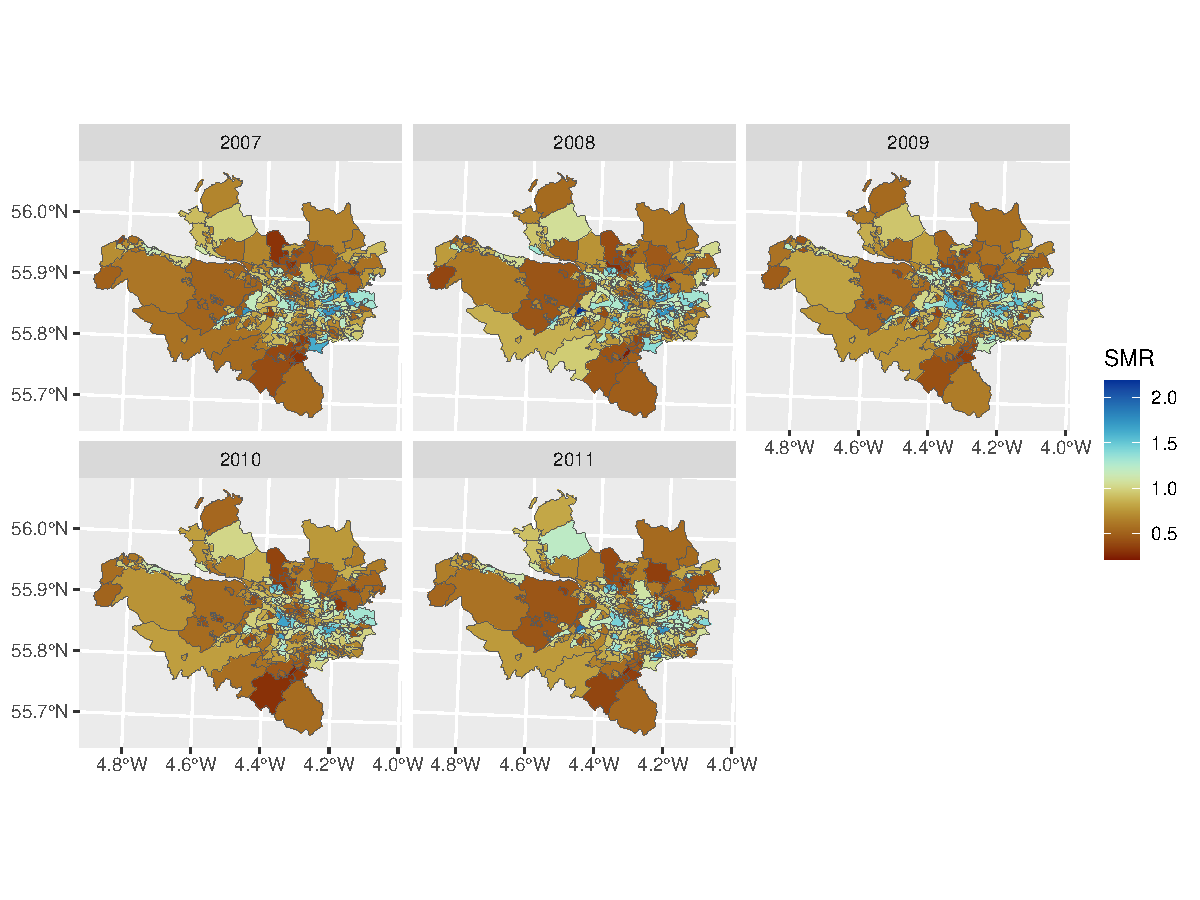
\includegraphics[keepaspectratio]{day4_practical_6_files/figure-pdf/unnamed-chunk-7-1.pdf}}

}

\caption{Bayesian residual plots: the left panel is the residual index
plot; the right panel is the plot of the residual versus the covariate
x}

\end{figure}%

We can also compare these against the theoretical quantiles of the
Normal distribution as follows:

\begin{Shaded}
\begin{Highlighting}[]
\FunctionTok{arrange}\NormalTok{(res\_samples, mean) }\SpecialCharTok{\%\textgreater{}\%}
  \FunctionTok{mutate}\NormalTok{(}\AttributeTok{theortical\_quantiles =} \FunctionTok{qnorm}\NormalTok{(}\DecValTok{1}\SpecialCharTok{:}\DecValTok{100} \SpecialCharTok{/}\NormalTok{ (}\DecValTok{1}\SpecialCharTok{+}\DecValTok{100}\NormalTok{))) }\SpecialCharTok{\%\textgreater{}\%}
  \FunctionTok{ggplot}\NormalTok{(}\FunctionTok{aes}\NormalTok{(}\AttributeTok{x=}\NormalTok{theortical\_quantiles,}\AttributeTok{y=}\NormalTok{ mean)) }\SpecialCharTok{+} 
  \FunctionTok{geom\_ribbon}\NormalTok{(}\FunctionTok{aes}\NormalTok{(}\AttributeTok{ymin =}\NormalTok{ q0}\FloatTok{.025}\NormalTok{, }\AttributeTok{ymax =}\NormalTok{ q0}\FloatTok{.975}\NormalTok{), }\AttributeTok{fill =} \StringTok{"grey70"}\NormalTok{)}\SpecialCharTok{+}
  \FunctionTok{geom\_abline}\NormalTok{(}\AttributeTok{intercept =} \FunctionTok{mean}\NormalTok{(res\_samples}\SpecialCharTok{$}\NormalTok{mean),}
              \AttributeTok{slope =} \FunctionTok{sd}\NormalTok{(res\_samples}\SpecialCharTok{$}\NormalTok{mean)) }\SpecialCharTok{+}
  \FunctionTok{geom\_point}\NormalTok{() }\SpecialCharTok{+}
  \FunctionTok{labs}\NormalTok{(}\AttributeTok{x =} \StringTok{"Theoretical Quantiles (Normal)"}\NormalTok{,}
       \AttributeTok{y=} \StringTok{"Sample Quantiles (Residuals)"}\NormalTok{) }
\end{Highlighting}
\end{Shaded}

\begin{center}
\pandocbounded{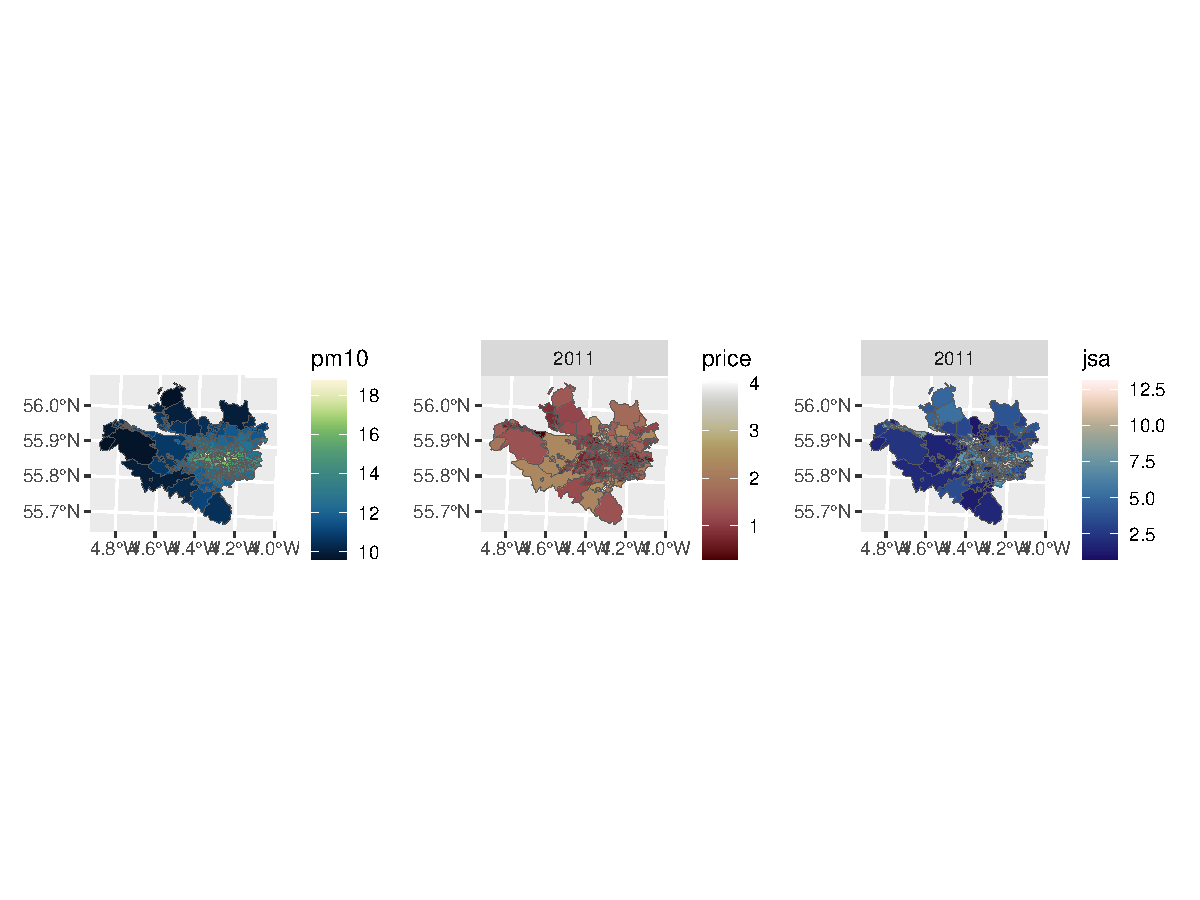
\includegraphics[keepaspectratio]{day4_practical_6_files/figure-pdf/unnamed-chunk-8-1.pdf}}
\end{center}

\subsubsection{Posterior Predictive
Checks}\label{posterior-predictive-checks}

Now, instead of generating samples from the mean, we will account for
the observational process uncertainty by:

\begin{enumerate}
\def\labelenumi{\arabic{enumi}.}
\tightlist
\item
  Sampling \(y^{1k}_i\sim\pi(y_i|\mathbf{y})\)
  \(k = 1,\dots,M;~i = 1,\ldots,100\) using \texttt{generate()} (here we
  will draw \(M=500\) samples)
\end{enumerate}

\begin{Shaded}
\begin{Highlighting}[]
\NormalTok{samples }\OtherTok{=}  \FunctionTok{generate}\NormalTok{(fit.lm, df,}
  \AttributeTok{formula =} \SpecialCharTok{\textasciitilde{}}\NormalTok{ \{}
\NormalTok{    mu }\OtherTok{\textless{}{-}}\NormalTok{ (beta\_0 }\SpecialCharTok{+}\NormalTok{ beta\_1)}
\NormalTok{    sd }\OtherTok{\textless{}{-}} \FunctionTok{sqrt}\NormalTok{(}\DecValTok{1} \SpecialCharTok{/}\NormalTok{ Precision\_for\_the\_Gaussian\_observations)}
    \FunctionTok{rnorm}\NormalTok{(}\DecValTok{100}\NormalTok{, }\AttributeTok{mean =}\NormalTok{ mu, }\AttributeTok{sd =}\NormalTok{ sd)}
\NormalTok{  \},}
  \AttributeTok{n.samples =} \DecValTok{500}
\NormalTok{) }
\end{Highlighting}
\end{Shaded}

\begin{enumerate}
\def\labelenumi{\arabic{enumi}.}
\setcounter{enumi}{1}
\tightlist
\item
  Comparing some summaries of the simulated data with the one of the
  observed one
\end{enumerate}

Here we compare (i) the estimated posterior densities
\(\hat{\pi}^k(y|\mathbf{y})\) with the estimated data density and (ii)
the samples means and 95\% credible intervals against the observations.

\begin{Shaded}
\begin{Highlighting}[]
\CommentTok{\# Tidy format for plotting}
\NormalTok{samples\_long }\OtherTok{=} \FunctionTok{data.frame}\NormalTok{(samples) }\SpecialCharTok{\%\textgreater{}\%} 
  \FunctionTok{mutate}\NormalTok{(}\AttributeTok{id =} \DecValTok{1}\SpecialCharTok{:}\DecValTok{100}\NormalTok{) }\SpecialCharTok{\%\textgreater{}\%} \CommentTok{\# i{-}th observation}
  \FunctionTok{pivot\_longer}\NormalTok{(}\SpecialCharTok{{-}}\NormalTok{id)}

\CommentTok{\# compute the mean and quantiles for the samples}
\NormalTok{draws\_summaries }\OtherTok{=} \FunctionTok{data.frame}\NormalTok{(}\AttributeTok{mean\_samples =} \FunctionTok{apply}\NormalTok{(samples,}\DecValTok{1}\NormalTok{,mean),}
\AttributeTok{q25 =} \FunctionTok{apply}\NormalTok{(samples,}\DecValTok{1}\NormalTok{,}\ControlFlowTok{function}\NormalTok{(x)}\FunctionTok{quantile}\NormalTok{(x,}\FloatTok{0.025}\NormalTok{)),  }
\AttributeTok{q975 =} \FunctionTok{apply}\NormalTok{(samples,}\DecValTok{1}\NormalTok{,}\ControlFlowTok{function}\NormalTok{(x)}\FunctionTok{quantile}\NormalTok{(x,}\FloatTok{0.975}\NormalTok{)),}
\AttributeTok{observations =}\NormalTok{ df}\SpecialCharTok{$}\NormalTok{y)  }

\NormalTok{p1 }\OtherTok{=} \FunctionTok{ggplot}\NormalTok{() }\SpecialCharTok{+} \FunctionTok{geom\_density}\NormalTok{(}\AttributeTok{data =}\NormalTok{ samples\_long, }
                        \FunctionTok{aes}\NormalTok{(value, }\AttributeTok{group =}\NormalTok{ name),  }\AttributeTok{color =} \StringTok{"\#E69F00"}\NormalTok{) }\SpecialCharTok{+}
  \FunctionTok{geom\_density}\NormalTok{(}\AttributeTok{data =}\NormalTok{ df, }\FunctionTok{aes}\NormalTok{(y))  }\SpecialCharTok{+}
  \FunctionTok{xlab}\NormalTok{(}\StringTok{""}\NormalTok{) }\SpecialCharTok{+} \FunctionTok{ylab}\NormalTok{(}\StringTok{""}\NormalTok{) }

\NormalTok{p2 }\OtherTok{=} \FunctionTok{ggplot}\NormalTok{(draws\_summaries,}\FunctionTok{aes}\NormalTok{(}\AttributeTok{y=}\NormalTok{mean\_samples,}\AttributeTok{x=}\NormalTok{observations))}\SpecialCharTok{+}
  \FunctionTok{geom\_errorbar}\NormalTok{(}\FunctionTok{aes}\NormalTok{(}\AttributeTok{ymin =}\NormalTok{ q25,}
                   \AttributeTok{ymax =}\NormalTok{ q975), }
               \AttributeTok{alpha =} \FloatTok{0.5}\NormalTok{, }\AttributeTok{color =} \StringTok{"grey50"}\NormalTok{)}\SpecialCharTok{+}
\FunctionTok{geom\_point}\NormalTok{()}\SpecialCharTok{+}\FunctionTok{geom\_abline}\NormalTok{(}\AttributeTok{slope =} \DecValTok{1}\NormalTok{,}\AttributeTok{intercept =} \DecValTok{0}\NormalTok{,}\AttributeTok{lty=}\DecValTok{2}\NormalTok{)}\SpecialCharTok{+}\FunctionTok{labs}\NormalTok{()}

\NormalTok{p1 }\SpecialCharTok{+}\NormalTok{p2}
\end{Highlighting}
\end{Shaded}

\pandocbounded{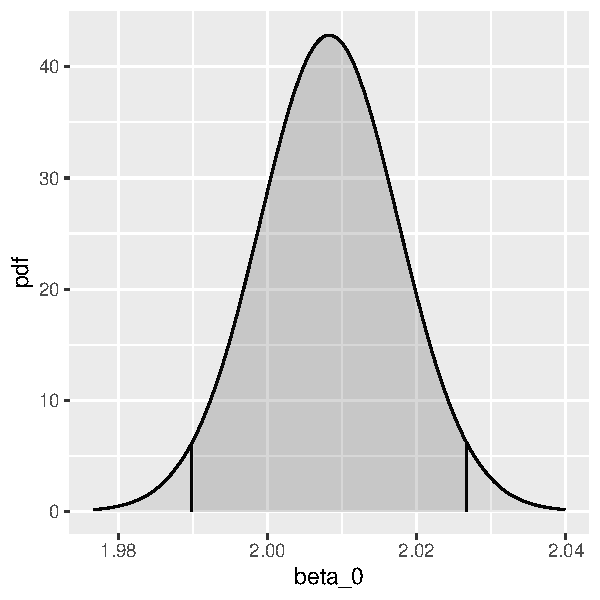
\includegraphics[keepaspectratio]{day4_practical_6_files/figure-pdf/unnamed-chunk-10-1.pdf}}

\subsection{GLM model checking}\label{sec-linmodel}

In this exercise we will:

\begin{itemize}
\tightlist
\item
  Learn about some model assessments techniques available in INLA
\item
  Conduct posterior predictive model checking using CPO and PIT
\end{itemize}

Libraries to load:

\begin{Shaded}
\begin{Highlighting}[]
\FunctionTok{library}\NormalTok{(dplyr)}
\FunctionTok{library}\NormalTok{(INLA)}
\FunctionTok{library}\NormalTok{(ggplot2)}
\FunctionTok{library}\NormalTok{(patchwork)}
\FunctionTok{library}\NormalTok{(inlabru)     }
\end{Highlighting}
\end{Shaded}

In this exercise, we will use data on horseshoe crabs (\emph{Limulus
polyphemus}) where the number of satellites males surrounding a breeding
female are counted along with the female's color and carapace width.

A possible model to study the factors that affect the number of
satellites for female crabs is

\[
\begin{aligned}
y_i&\sim\mathrm{Poisson}(\mu_i), \qquad i = 1,\dots,N \\
\eta_i &= \mu_i = \beta_0 + \beta_1 x_i + \ldots
\end{aligned}
\]

We can explore the conditional means and variances given the female's
color:

\begin{Shaded}
\begin{Highlighting}[]
\NormalTok{crabs }\OtherTok{\textless{}{-}} \FunctionTok{read.csv}\NormalTok{(}\StringTok{"datasets/crabs.csv"}\NormalTok{)}

\CommentTok{\# conditional means and variances}
\NormalTok{crabs }\SpecialCharTok{\%\textgreater{}\%}
  \FunctionTok{summarise}\NormalTok{( }\AttributeTok{Mean =} \FunctionTok{mean}\NormalTok{(satell ),}
             \AttributeTok{Variance =} \FunctionTok{var}\NormalTok{(satell),}
                     \AttributeTok{.by =}\NormalTok{ color)}
\end{Highlighting}
\end{Shaded}

\begin{verbatim}
   color     Mean  Variance
1 medium 3.294737 10.273908
2   dark 2.227273  6.737844
3  light 4.083333  9.719697
4 darker 2.045455 13.093074
\end{verbatim}

The mean of the number of satellites vary by color which gives a good
indication that color might be useful for predicting satellites numbers.
However, notice that the mean is lower than its variance suggesting that
overdispersion might be present and that a negative binomial model would
be more appropriate for the data (we will cover this later).

\textbf{Fitting the model}

First, lets begin fitting the Poisson model above using the carapace's
color and width as predictors. Since, color is a categorical variable in
our model we need to create a dummy variable for it. We can use the
\texttt{model.matrix} function to help us constructing the design matrix
and then append this to our data:

\begin{Shaded}
\begin{Highlighting}[]
\NormalTok{crabs\_df }\OtherTok{=} \FunctionTok{model.matrix}\NormalTok{( }\SpecialCharTok{\textasciitilde{}}\NormalTok{  color , crabs) }\SpecialCharTok{\%\textgreater{}\%}
  \FunctionTok{as.data.frame}\NormalTok{() }\SpecialCharTok{\%\textgreater{}\%}
  \FunctionTok{select}\NormalTok{(}\SpecialCharTok{{-}}\DecValTok{1}\NormalTok{) }\SpecialCharTok{\%\textgreater{}\%}        \CommentTok{\# drop intercept}
  \FunctionTok{bind\_cols}\NormalTok{(crabs) }\SpecialCharTok{\%\textgreater{}\%}  \CommentTok{\# append to original data}
  \FunctionTok{select}\NormalTok{(}\SpecialCharTok{{-}}\NormalTok{color)        }\CommentTok{\# remove original color categorical variable}
\end{Highlighting}
\end{Shaded}

The new data set \texttt{crabs\_df} contains a dummy variable for the
different color categories (\texttt{dark} being the reference category).
Then we can fit the model in \texttt{inlabru} as follows:

\begin{Shaded}
\begin{Highlighting}[]
\NormalTok{cmp }\OtherTok{=}  \ErrorTok{\textasciitilde{}} \SpecialCharTok{{-}}\DecValTok{1} \SpecialCharTok{+} \FunctionTok{beta0}\NormalTok{(}\DecValTok{1}\NormalTok{) }\SpecialCharTok{+}\NormalTok{  colordarker }\SpecialCharTok{+}
\NormalTok{       colorlight }\SpecialCharTok{+}\NormalTok{ colormedium }\SpecialCharTok{+}
       \FunctionTok{w}\NormalTok{(weight, }\AttributeTok{model =} \StringTok{"linear"}\NormalTok{)}

\NormalTok{lik }\OtherTok{=}  \FunctionTok{bru\_obs}\NormalTok{(}\AttributeTok{formula =}\NormalTok{ satell }\SpecialCharTok{\textasciitilde{}}\NormalTok{.,}
            \AttributeTok{family =} \StringTok{"poisson"}\NormalTok{,}
            \AttributeTok{data =}\NormalTok{ crabs\_df)}

\NormalTok{fit\_pois }\OtherTok{=} \FunctionTok{bru}\NormalTok{(cmp, lik)}

\FunctionTok{summary}\NormalTok{(fit\_pois)}
\end{Highlighting}
\end{Shaded}

\begin{verbatim}
inlabru version: 2.13.0
INLA version: 25.08.21-1
Components:
beta0: main = linear(1), group = exchangeable(1L), replicate = iid(1L), NULL
colordarker: main = linear(colordarker), group = exchangeable(1L), replicate = iid(1L), NULL
colorlight: main = linear(colorlight), group = exchangeable(1L), replicate = iid(1L), NULL
colormedium: main = linear(colormedium), group = exchangeable(1L), replicate = iid(1L), NULL
w: main = linear(weight), group = exchangeable(1L), replicate = iid(1L), NULL
Observation models:
  Family: 'poisson'
    Tag: <No tag>
    Data class: 'data.frame'
    Response class: 'integer'
    Predictor: satell ~ .
    Additive/Linear: TRUE/TRUE
    Used components: effects[beta0, colordarker, colorlight, colormedium, w], latent[]
Time used:
    Pre = 0.334, Running = 0.264, Post = 0.0784, Total = 0.676 
Fixed effects:
              mean    sd 0.025quant 0.5quant 0.975quant   mode kld
beta0       -0.501 0.196     -0.885   -0.501     -0.117 -0.501   0
colordarker -0.008 0.180     -0.362   -0.008      0.345 -0.008   0
colorlight   0.445 0.176      0.101    0.445      0.790  0.445   0
colormedium  0.248 0.118      0.017    0.248      0.479  0.248   0
w            0.001 0.000      0.000    0.001      0.001  0.001   0

Marginal log-Likelihood:  -489.43 
 is computed 
Posterior summaries for the linear predictor and the fitted values are computed
(Posterior marginals needs also 'control.compute=list(return.marginals.predictor=TRUE)')
\end{verbatim}

\subsubsection{Model assessment and model
choice}\label{model-assessment-and-model-choice}

Now that we have fitted the model we would like to carry some model
assessments. In a Bayesian setting, this is often based on posterior
predictive checks. To do so, we will use the CPO and PIT - two commonly
used Bayesian model assessment criteria based on the \textbf{posterior
predictive distribution}.

\begin{tcolorbox}[enhanced jigsaw, opacitybacktitle=0.6, breakable, bottomrule=.15mm, rightrule=.15mm, left=2mm, leftrule=.75mm, toptitle=1mm, colframe=quarto-callout-note-color-frame, opacityback=0, toprule=.15mm, colback=white, arc=.35mm, title=\textcolor{quarto-callout-note-color}{\faInfo}\hspace{0.5em}{Posterior predictive model checking}, coltitle=black, colbacktitle=quarto-callout-note-color!10!white, titlerule=0mm, bottomtitle=1mm]

The posterior predictive distribution for a predicted value \(\hat{y}\)
is

\[
\pi(\hat{y}|\mathbf{y}) = \int_\theta \pi(\hat{y}|\theta)\pi(\theta|\mathbf{y})d\theta.
\]

The probability integral transform (PIT) introduced by Dawid (1984) is
defined for each observation as:

\[
\mathrm{PIT}_i = \pi(\hat{y}_i \leq y_i |\mathbf{y}{-i})
\]

The PIT evaluates how well a model's predicted values match the observed
data distribution. It is computed as the cumulative distribution
function (CDF) of the observed data evaluated at each predicted value.
If the model is well-calibrated, the PIT values should be
\emph{approximately uniformly distributed}. Deviations from this uniform
distribution may indicate issues with model calibration or overfitting.

Another metric we could used to asses the model fit is the conditional
predictive ordinate (CPO) introduced by Pettit (1990), and defined as:

\[
\text{CPO}_i = \pi(y_i| \mathbf{y}{-i})
\]

The CPO measures the density of the observed value of \(y_i\) when model
is fit using all data but \(y_i\). CPO provides a measure of how well
the model predicts each individual observation while taking into account
the rest of the data and the model. \emph{Large values indicate a better
fit} of the model to the data, while small values indicate a bad fitting
of the model

\end{tcolorbox}

To compute PIT and CPO we can either:

\begin{enumerate}
\def\labelenumi{\arabic{enumi}.}
\item
  ask \texttt{inlabru} to compute them by set
  \texttt{options\ =\ list(control.compute\ =\ list(cpo\ =\ TRUE))} in
  the \texttt{bru()} function arguments.
\item
  set this as default in \texttt{inlabru} global option using the
  \texttt{bru\_options\_set} function.
\end{enumerate}

Here we will do the later and re-run the model

\begin{Shaded}
\begin{Highlighting}[]
\FunctionTok{bru\_options\_set}\NormalTok{(}\AttributeTok{control.compute =} \FunctionTok{list}\NormalTok{(}\AttributeTok{cpo =} \ConstantTok{TRUE}\NormalTok{))}

\NormalTok{fit\_pois }\OtherTok{=} \FunctionTok{bru}\NormalTok{(cmp, lik)}
\end{Highlighting}
\end{Shaded}

Now we can produce histograms and QQ plots to assess for uniformity in
the PIT values which can be accessed through
\texttt{inlabru\_model\$cpo\$pit} :

\section{Plot}

\begin{center}
\pandocbounded{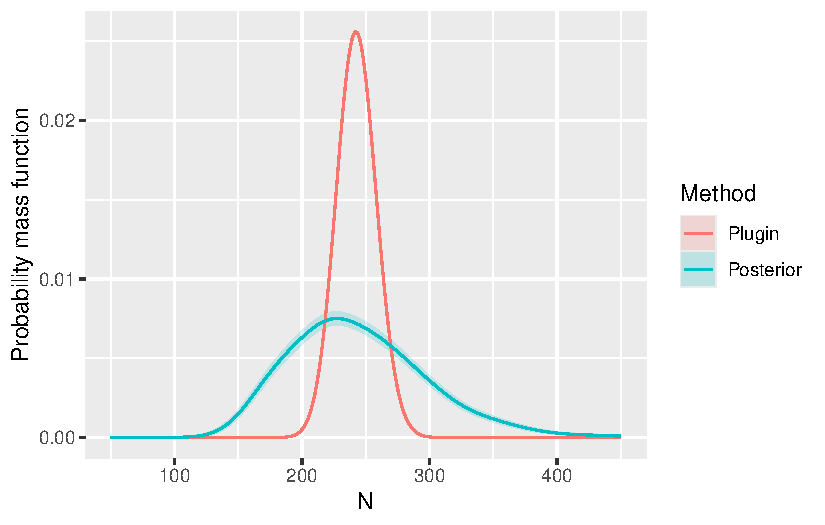
\includegraphics[keepaspectratio]{day4_practical_6_files/figure-pdf/unnamed-chunk-27-1.pdf}}
\end{center}

\section{R Code}

\begin{Shaded}
\begin{Highlighting}[]
\NormalTok{fit\_pois}\SpecialCharTok{$}\NormalTok{cpo}\SpecialCharTok{$}\NormalTok{pit }\SpecialCharTok{\%\textgreater{}\%}
  \FunctionTok{hist}\NormalTok{(}\AttributeTok{main =} \StringTok{"Histogram of PIT values"}\NormalTok{)}

\FunctionTok{qqplot}\NormalTok{(}\FunctionTok{qunif}\NormalTok{(}\FunctionTok{ppoints}\NormalTok{(}\FunctionTok{length}\NormalTok{(fit\_pois}\SpecialCharTok{$}\NormalTok{cpo}\SpecialCharTok{$}\NormalTok{pit))),}
\NormalTok{       fit\_pois}\SpecialCharTok{$}\NormalTok{cpo}\SpecialCharTok{$}\NormalTok{pit,}
       \AttributeTok{main =} \StringTok{"Q{-}Q plot for Unif(0,1)"}\NormalTok{,}
       \AttributeTok{xlab =} \StringTok{"Theoretical Quantiles"}\NormalTok{,}
       \AttributeTok{ylab =} \StringTok{"Sample Quantiles"}\NormalTok{)}

\FunctionTok{qqline}\NormalTok{(fit\_pois}\SpecialCharTok{$}\NormalTok{cpo}\SpecialCharTok{$}\NormalTok{pit,}
       \AttributeTok{distribution =} \ControlFlowTok{function}\NormalTok{(p) }\FunctionTok{qunif}\NormalTok{(p),}
       \AttributeTok{prob =} \FunctionTok{c}\NormalTok{(}\FloatTok{0.1}\NormalTok{, }\FloatTok{0.9}\NormalTok{))}
\end{Highlighting}
\end{Shaded}

Both Q-Q plots and histogram of the PIT values suggest a not so great
model fit. For the CPO values, usually the following summary of the CPO
is often used:

\[
-\sum_{i=1}^n \log (\text{CPO}\_i)
\]

This quantities is useful when comparing different models - a smaller
values indicate a better model fit. CPO values can be accessed by typing
\texttt{inlabru\_model\$cpo\$cpo}.

\begin{tcolorbox}[enhanced jigsaw, opacitybacktitle=0.6, breakable, bottomrule=.15mm, rightrule=.15mm, left=2mm, leftrule=.75mm, toptitle=1mm, colframe=quarto-callout-warning-color-frame, opacityback=0, toprule=.15mm, colback=white, arc=.35mm, title={Task}, coltitle=black, colbacktitle=quarto-callout-warning-color!10!white, titlerule=0mm, bottomtitle=1mm]

The model assessment above suggests that a Poisson model might not be
the most appropriate model, likely due to the overdispersion we detected
previously. Fit a Negative binomial to relax the Poisson model
assumption that the conditional mean and variance are equal. Then,
compute the CPO summary statistic and PIT QQ plot to decide which model
gives the better fit.

Take hint

To specify a negative binomial model you only need to change the family
distribution to \texttt{family\ =\ \ "nbinomial"}.

Click here to see the solution

\begin{Shaded}
\begin{Highlighting}[]
\FunctionTok{par}\NormalTok{(}\AttributeTok{mfrow=}\FunctionTok{c}\NormalTok{(}\DecValTok{1}\NormalTok{,}\DecValTok{2}\NormalTok{))}

\CommentTok{\# Fit the negative binomial model}

\NormalTok{lik\_nbinom }\OtherTok{=}  \FunctionTok{bru\_obs}\NormalTok{(}\AttributeTok{formula =}\NormalTok{ satell }\SpecialCharTok{\textasciitilde{}}\NormalTok{.,}
            \AttributeTok{family =} \StringTok{"nbinomial"}\NormalTok{,}
            \AttributeTok{data =}\NormalTok{ crabs\_df)}

\NormalTok{fit\_nbinom }\OtherTok{=} \FunctionTok{bru}\NormalTok{(cmp, lik\_nbinom)}

\CommentTok{\# PIT checks}

\NormalTok{fit\_nbinom}\SpecialCharTok{$}\NormalTok{cpo}\SpecialCharTok{$}\NormalTok{pit }\SpecialCharTok{\%\textgreater{}\%}
  \FunctionTok{hist}\NormalTok{(}\AttributeTok{main =} \StringTok{"Histogram of PIT values"}\NormalTok{)}

\FunctionTok{qqplot}\NormalTok{(}\FunctionTok{qunif}\NormalTok{(}\FunctionTok{ppoints}\NormalTok{(}\FunctionTok{length}\NormalTok{(fit\_nbinom}\SpecialCharTok{$}\NormalTok{cpo}\SpecialCharTok{$}\NormalTok{pit))),}
\NormalTok{       fit\_nbinom}\SpecialCharTok{$}\NormalTok{cpo}\SpecialCharTok{$}\NormalTok{pit,}
       \AttributeTok{main =} \StringTok{"Q{-}Q plot for Unif(0,1)"}\NormalTok{,}
       \AttributeTok{xlab =} \StringTok{"Theoretical Quantiles"}\NormalTok{,}
       \AttributeTok{ylab =} \StringTok{"Sample Quantiles"}\NormalTok{)}

\FunctionTok{qqline}\NormalTok{(fit\_nbinom}\SpecialCharTok{$}\NormalTok{cpo}\SpecialCharTok{$}\NormalTok{pit,}
       \AttributeTok{distribution =} \ControlFlowTok{function}\NormalTok{(p) }\FunctionTok{qunif}\NormalTok{(p),}
       \AttributeTok{prob =} \FunctionTok{c}\NormalTok{(}\FloatTok{0.1}\NormalTok{, }\FloatTok{0.9}\NormalTok{))}
\end{Highlighting}
\end{Shaded}

\begin{center}
\pandocbounded{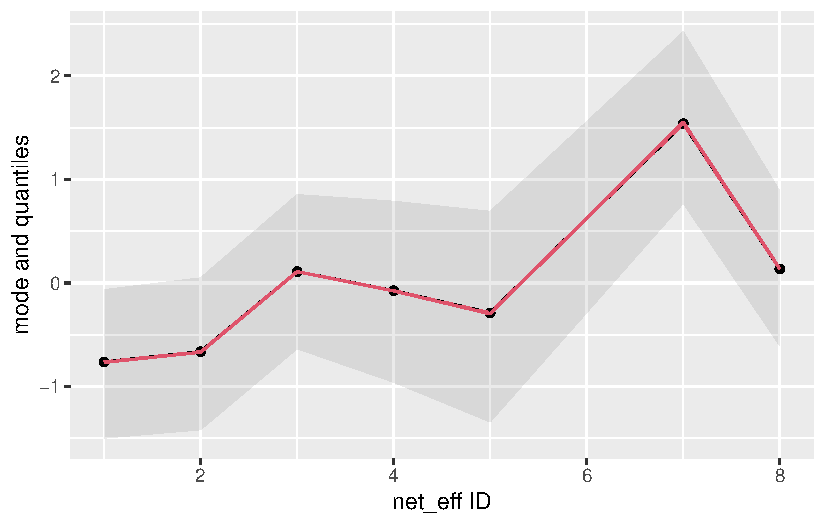
\includegraphics[keepaspectratio]{day4_practical_6_files/figure-pdf/unnamed-chunk-29-1.pdf}}
\end{center}

\begin{Shaded}
\begin{Highlighting}[]
\CommentTok{\# CPO comparison}

\FunctionTok{data.frame}\NormalTok{( }\AttributeTok{CPO =} \FunctionTok{c}\NormalTok{(}\SpecialCharTok{{-}}\FunctionTok{sum}\NormalTok{(}\FunctionTok{log}\NormalTok{(fit\_pois}\SpecialCharTok{$}\NormalTok{cpo}\SpecialCharTok{$}\NormalTok{cpo)),}
                    \SpecialCharTok{{-}}\FunctionTok{sum}\NormalTok{(}\FunctionTok{log}\NormalTok{(fit\_nbinom}\SpecialCharTok{$}\NormalTok{cpo}\SpecialCharTok{$}\NormalTok{cpo))),}
          \AttributeTok{Model =} \FunctionTok{c}\NormalTok{(}\StringTok{"Poisson"}\NormalTok{,}\StringTok{"Negative Binomial"}\NormalTok{))}
\end{Highlighting}
\end{Shaded}

\begin{verbatim}
       CPO             Model
1 465.4061           Poisson
2 379.3340 Negative Binomial
\end{verbatim}

\begin{Shaded}
\begin{Highlighting}[]
\CommentTok{\# Overall, we can see that the negative binomial model provides a better fit to the data.}
\end{Highlighting}
\end{Shaded}

\end{tcolorbox}

\subsection{Leave-Group-Out Cross
validation}\label{leave-group-out-cross-validation}

In this practical we are going to fit a geostatistical model. We will:

\begin{itemize}
\tightlist
\item
  Learn how to to compute model comparison in \texttt{inlabru} using
  LGOCV
\end{itemize}

\begin{center}\rule{0.5\linewidth}{0.5pt}\end{center}

Libraries to load:

\begin{Shaded}
\begin{Highlighting}[]
\FunctionTok{library}\NormalTok{(dplyr)}
\FunctionTok{library}\NormalTok{(INLA)}
\FunctionTok{library}\NormalTok{(inlabru) }
\FunctionTok{library}\NormalTok{(sf)}
\FunctionTok{library}\NormalTok{(terra)}


\CommentTok{\# load some libraries to generate nice map plots}
\FunctionTok{library}\NormalTok{(scico)}
\FunctionTok{library}\NormalTok{(ggplot2)}
\FunctionTok{library}\NormalTok{(patchwork)}
\FunctionTok{library}\NormalTok{(mapview)}
\FunctionTok{library}\NormalTok{(tidyterra)}
\end{Highlighting}
\end{Shaded}

\subsubsection{The data}\label{the-data}

In this practical, we will revisit the data on the Pacific Cod
(\emph{Gadus macrocephalus}) from a trawl survey in Queen Charlotte
Sound. The \texttt{pcod} dataset is available from the \texttt{sdmTMB}
package and contains the presence/absence records of the Pacific Cod
during each surveys along with the biomass density of Pacific cod in the
area swept (kg/Km\(^2\)). The \texttt{qcs\_grid} data contain the depth
values stored as \(2\times 2\) km grid for Queen Charlotte Sound.

The dataset contains presence/absence data from 2003 to 2017. Lets
consider year 2003 for now.

We first load the dataset and select the year of interest

\begin{Shaded}
\begin{Highlighting}[]
\FunctionTok{library}\NormalTok{(sdmTMB)}

\NormalTok{pcod\_df }\OtherTok{=}\NormalTok{ sdmTMB}\SpecialCharTok{::}\NormalTok{pcod }\SpecialCharTok{\%\textgreater{}\%} \FunctionTok{filter}\NormalTok{(year}\SpecialCharTok{==}\DecValTok{2003}\NormalTok{)}
\NormalTok{qcs\_grid }\OtherTok{=}\NormalTok{ sdmTMB}\SpecialCharTok{::}\NormalTok{qcs\_grid}
\end{Highlighting}
\end{Shaded}

Then, we create ab \texttt{sf} object and assign the rough coordinate
reference to it:

\begin{Shaded}
\begin{Highlighting}[]
\NormalTok{pcod\_sf }\OtherTok{=}   \FunctionTok{st\_as\_sf}\NormalTok{(pcod\_df, }\AttributeTok{coords =} \FunctionTok{c}\NormalTok{(}\StringTok{"lon"}\NormalTok{,}\StringTok{"lat"}\NormalTok{), }\AttributeTok{crs =} \DecValTok{4326}\NormalTok{)}
\NormalTok{pcod\_sf }\OtherTok{=} \FunctionTok{st\_transform}\NormalTok{(pcod\_sf,}
          \AttributeTok{crs =} \StringTok{"+proj=utm +zone=9 +datum=WGS84 +no\_defs +type=crs +units=km"}\NormalTok{ )}
\end{Highlighting}
\end{Shaded}

We convert the covariate into a raster and assign the same coordinate
reference:

\begin{Shaded}
\begin{Highlighting}[]
\NormalTok{depth\_r }\OtherTok{\textless{}{-}} \FunctionTok{rast}\NormalTok{(qcs\_grid, }\AttributeTok{type =} \StringTok{"xyz"}\NormalTok{)}
\FunctionTok{crs}\NormalTok{(depth\_r) }\OtherTok{\textless{}{-}} \FunctionTok{crs}\NormalTok{(pcod\_sf)}
\end{Highlighting}
\end{Shaded}

\begin{center}
\pandocbounded{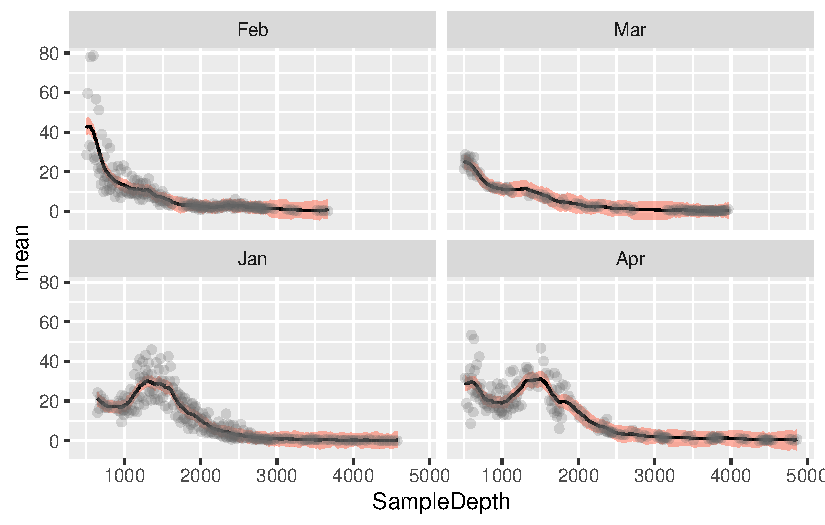
\includegraphics[keepaspectratio]{day4_practical_6_files/figure-pdf/unnamed-chunk-46-1.pdf}}
\end{center}

\subsubsection{The models}\label{the-models}

Here, we will model the binary presence-absence data as a Binomial model
of the form:

\[
\begin{aligned}
y(s)|\eta(s)&\sim\text{Binom}(1, p(s))\\
\eta(s) &= \text{logit}(p(s)) \\
\omega(s) &\sim \text{  GF with range } \rho\  \text{ and maginal variance }\ \sigma^2
\end{aligned}
\]

We will fit three models. One where we consider the observation as
Bernoulli and where the linear predictor contains only one intercept and
the GR field \(\omega(s)\) defined through the SPDE approach. The other
two models will also include depth as a linear and non-linear smoothed
covariate in the linear predictor.

\textbf{Construct the mesh and the SPDE model}

\begin{Shaded}
\begin{Highlighting}[]
\NormalTok{mesh }\OtherTok{=} \FunctionTok{fm\_mesh\_2d}\NormalTok{(}\AttributeTok{loc =}\NormalTok{ pcod\_sf,         }
                  \AttributeTok{max.edge =} \FunctionTok{c}\NormalTok{(}\DecValTok{10}\NormalTok{,}\DecValTok{20}\NormalTok{),     }
                  \AttributeTok{offset =} \FunctionTok{c}\NormalTok{(}\DecValTok{5}\NormalTok{,}\DecValTok{50}\NormalTok{))   }

\NormalTok{spde\_model }\OtherTok{=}  \FunctionTok{inla.spde2.pcmatern}\NormalTok{(mesh,}
                                  \AttributeTok{prior.sigma =} \FunctionTok{c}\NormalTok{(}\DecValTok{1}\NormalTok{, }\FloatTok{0.5}\NormalTok{),}
                                  \AttributeTok{prior.range =} \FunctionTok{c}\NormalTok{(}\DecValTok{100}\NormalTok{, }\FloatTok{0.5}\NormalTok{))}
\end{Highlighting}
\end{Shaded}

\begin{center}
\pandocbounded{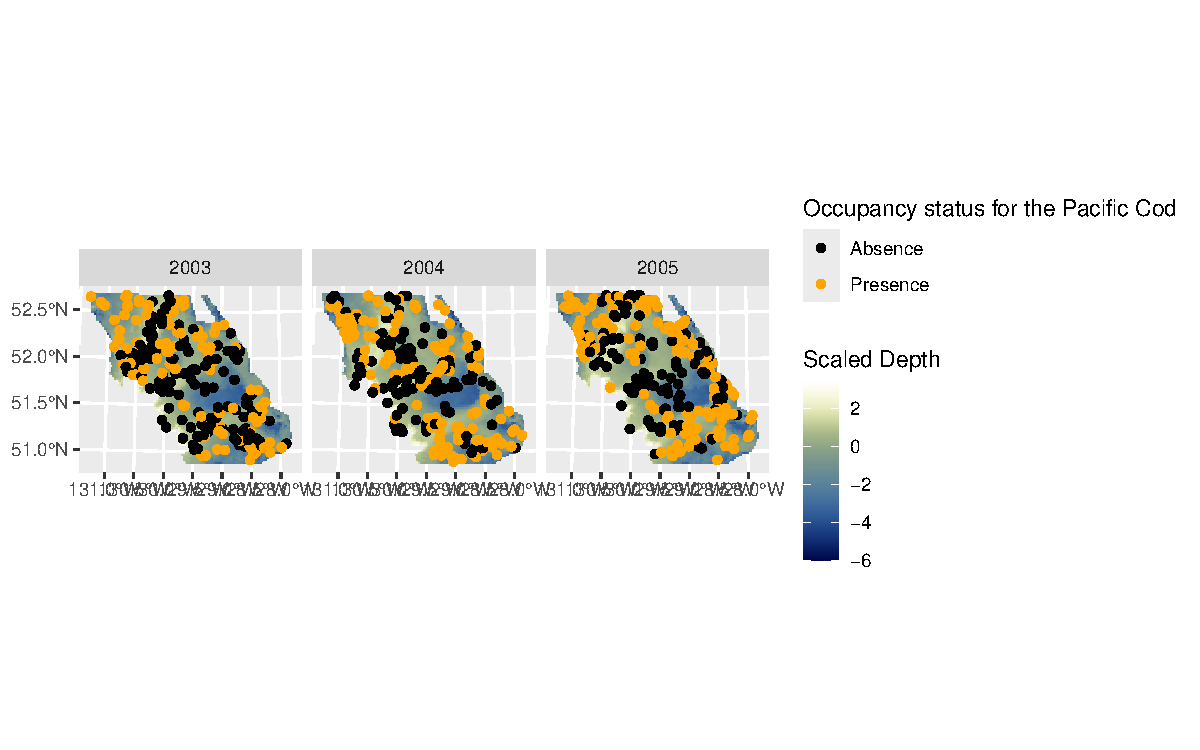
\includegraphics[keepaspectratio]{day4_practical_6_files/figure-pdf/unnamed-chunk-48-1.pdf}}
\end{center}

\textbf{Model 1 - spatial only}

\begin{enumerate}
\def\labelenumi{\arabic{enumi}.}
\tightlist
\item
  \textbf{Model 1 - spatial only} This is a model with that includes a
  structured spatial effect only. Here the linear predictor is defined
  as:
\end{enumerate}

\[
  \eta(s) = \text{logit}(p(s)) = \beta_0 + \omega(s) 
\]

\begin{Shaded}
\begin{Highlighting}[]
\CommentTok{\# Model 1 components}
\NormalTok{cmp\_1 }\OtherTok{=} \ErrorTok{\textasciitilde{}} \FunctionTok{Intercept}\NormalTok{(}\DecValTok{1}\NormalTok{) }\SpecialCharTok{+} \FunctionTok{space}\NormalTok{(geometry, }\AttributeTok{model =}\NormalTok{ spde\_model)}

\CommentTok{\# Model 1 linear predictor}
\NormalTok{formula\_1 }\OtherTok{=}\NormalTok{ present }\SpecialCharTok{\textasciitilde{}}\NormalTok{ Intercept  }\SpecialCharTok{+}\NormalTok{ space}

\CommentTok{\# Model 1 observational model}
\NormalTok{lik\_1 }\OtherTok{=} \FunctionTok{bru\_obs}\NormalTok{(}\AttributeTok{formula =}\NormalTok{ formula\_1, }
              \AttributeTok{data =}\NormalTok{ pcod\_sf, }
              \AttributeTok{family =} \StringTok{"binomial"}\NormalTok{)}
\CommentTok{\# fit Model 1}
\NormalTok{fit\_spatial }\OtherTok{=} \FunctionTok{bru}\NormalTok{(cmp\_1,lik\_1)}
\end{Highlighting}
\end{Shaded}

\begin{enumerate}
\def\labelenumi{\arabic{enumi}.}
\setcounter{enumi}{1}
\tightlist
\item
  \textbf{Model 2 - Depth covariate} The depth enters the model in a
  linear way. The linear predictor is then defined as:
\end{enumerate}

\[
  \eta(s) = \text{logit}(p(s)) = \beta_0 + \omega(s) + \beta_1\ \text{depth}(s)
\]

\begin{Shaded}
\begin{Highlighting}[]
\CommentTok{\# Model 2 components}
\NormalTok{cmp\_2 }\OtherTok{=} \ErrorTok{\textasciitilde{}} \FunctionTok{Intercept}\NormalTok{(}\DecValTok{1}\NormalTok{) }\SpecialCharTok{+} 
  \FunctionTok{space}\NormalTok{(geometry, }\AttributeTok{model =}\NormalTok{ spde\_model)}\SpecialCharTok{+}
  \FunctionTok{covariate}\NormalTok{(depth\_r}\SpecialCharTok{$}\NormalTok{depth\_scaled, }\AttributeTok{model =} \StringTok{"linear"}\NormalTok{) }

\CommentTok{\# Model 2 linear predictor}
\NormalTok{formula\_2 }\OtherTok{=}\NormalTok{ present }\SpecialCharTok{\textasciitilde{}}\NormalTok{ Intercept  }\SpecialCharTok{+}\NormalTok{ covariate }\SpecialCharTok{+}\NormalTok{ space}

\CommentTok{\# Model 2 observational model}
\NormalTok{lik\_2 }\OtherTok{=} \FunctionTok{bru\_obs}\NormalTok{(}\AttributeTok{formula =}\NormalTok{ formula\_2, }
              \AttributeTok{data =}\NormalTok{ pcod\_sf, }
              \AttributeTok{family =} \StringTok{"binomial"}\NormalTok{)}

\CommentTok{\# Fit Model 2}
\NormalTok{fit\_depth\_linear }\OtherTok{=} \FunctionTok{bru}\NormalTok{(cmp\_2,lik\_2)}
\end{Highlighting}
\end{Shaded}

\begin{enumerate}
\def\labelenumi{\arabic{enumi}.}
\setcounter{enumi}{2}
\tightlist
\item
  \textbf{Model 2 - Smooth depth covariate} The depth enters the model
  in a non linear way. The linear predictor is then defined as:
\end{enumerate}

\[
  \eta(s) = \text{logit}(p(s)) = \beta_0 + \omega(s) +  f(\text{depth}(s))
\]

\begin{Shaded}
\begin{Highlighting}[]
\CommentTok{\# create the grouped variable}
\NormalTok{depth\_r}\SpecialCharTok{$}\NormalTok{depth\_group }\OtherTok{=} \FunctionTok{inla.group}\NormalTok{(}\FunctionTok{values}\NormalTok{(depth\_r}\SpecialCharTok{$}\NormalTok{depth\_scaled))}

\CommentTok{\# Model 3 components}
\NormalTok{cmp\_3 }\OtherTok{=} \ErrorTok{\textasciitilde{}} \FunctionTok{Intercept}\NormalTok{(}\DecValTok{1}\NormalTok{) }\SpecialCharTok{+} 
  \FunctionTok{space}\NormalTok{(geometry, }\AttributeTok{model =}\NormalTok{ spde\_model)}\SpecialCharTok{+}
  \FunctionTok{covariate}\NormalTok{(depth\_r}\SpecialCharTok{$}\NormalTok{depth\_group, }\AttributeTok{model =} \StringTok{"rw2"}\NormalTok{)}

\CommentTok{\# Model 3 linear predictor}
\NormalTok{formula\_3 }\OtherTok{=}\NormalTok{ present }\SpecialCharTok{\textasciitilde{}}\NormalTok{ Intercept  }\SpecialCharTok{+}\NormalTok{ covariate }\SpecialCharTok{+}\NormalTok{ space}

\CommentTok{\# Model 2 observational model}
\NormalTok{lik\_3 }\OtherTok{=} \FunctionTok{bru\_obs}\NormalTok{(}\AttributeTok{formula =}\NormalTok{ formula\_2, }
              \AttributeTok{data =}\NormalTok{ pcod\_sf, }
              \AttributeTok{family =} \StringTok{"binomial"}\NormalTok{)}

\CommentTok{\# Fit Model 2}
\NormalTok{fit\_depth\_smooth }\OtherTok{=} \FunctionTok{bru}\NormalTok{(cmp\_3,lik\_3)}
\end{Highlighting}
\end{Shaded}

\subsubsection{Model Comparison through
LGOCV}\label{model-comparison-through-lgocv}

Next we illustrate how to implement modelling comparison using leave-out
group cross validation (LGOCV). The underlying idea is that of a
Bayesian prediction setting where we approximate the posterior
predictive density \(\pi(\mathbf{\tilde{Y}}|\mathbf{y})\) defined as the
integral over the posterior distribution of the parameters, i.e.

\[
\pi(\mathbf{\tilde{Y}}|\mathbf{y}) = \int_\theta \pi(\mathbf{\tilde{Y}}|\theta,\mathbf{y}) \pi(\theta|\mathbf{y})d\theta
\]

the LGOCV selects a fixed test point \(i\) and remove a certain group of
data \(\mathbb{I}_i\) according to a specific prediction task. Thus, we
are interested in the posterior predictive density

\[
\pi(Y_i|\mathbf{y}{-\mathcal{I}i}) = \int\theta \pi(Y_i|\theta,\mathbf{y}{-\mathbb{I}_i}) \pi(\theta|\mathbf{y})d\theta
\]

With this, a point estimate \(\tilde{Y_i}\) can be computed based on
\(\pi(Y_i|\mathbf{y}_{-\mathbb{I}_i})\) and the predictive performance
be assessed using an appropriate scoring function
\(U(\tilde{Y}_i,Y_i)\), for example, the log-score function

\[
\frac{1}{n}\sum_{i=1}^n \mathrm{log}~ \pi(\mathbf{\tilde{y}}|\mathbf{y}).
\]

In this example, the LGOCV strategy will be used to compare the previous
fitted spatially explicit models. Here, the leave-out group
\(\mathbb{I}_i\) is manually defined for the \(i\)th row of the data
based on a buffer of size \(b=25\) centered at each data point:

\begin{Shaded}
\begin{Highlighting}[]
\CommentTok{\# create buffer of size 25 centred at each site}
\NormalTok{buffer }\OtherTok{\textless{}{-}} \FunctionTok{st\_buffer}\NormalTok{(pcod\_sf, }\AttributeTok{dist =} \DecValTok{25}\NormalTok{)}

\CommentTok{\# Lists of the indexes of the leave{-}out{-}group for each observation i}
\NormalTok{Ii }\OtherTok{\textless{}{-}} \FunctionTok{st\_intersects}\NormalTok{(pcod\_sf,buffer)}
\end{Highlighting}
\end{Shaded}

Figure~\ref{fig-cv_ex} illustrate the manual construction of the
leave-out-group for the 2nd observation in our data.

\begin{figure}

\centering{

\pandocbounded{\includegraphics[keepaspectratio]{day4_practical_6_files/figure-pdf/fig-cv_ex-1.pdf}}

}

\caption{\label{fig-cv_ex}Example of the CV strategy for the 2nd testing
point.}

\end{figure}%

We then can use the \texttt{inla.group.cv} function to compute the
log-scores for Model 3 as follows:

\begin{Shaded}
\begin{Highlighting}[]
\NormalTok{lgocv\_depth\_smooth }\OtherTok{=} \FunctionTok{inla.group.cv}\NormalTok{(}\AttributeTok{result =}\NormalTok{ fit\_depth\_smooth,}
                                   \AttributeTok{groups =}\NormalTok{ Ii)}
\NormalTok{log\_depth\_smooth }\OtherTok{=} \FunctionTok{mean}\NormalTok{(}\FunctionTok{log}\NormalTok{(lgocv\_depth\_smooth}\SpecialCharTok{$}\NormalTok{cv),}
                        \AttributeTok{na.rm=}\NormalTok{T)}
\end{Highlighting}
\end{Shaded}

When we do model comparison, we want to have the same groups for
different models. We can easily do this by passing an
\texttt{inla.group.cv} class object to \texttt{inla.group.cv}function.
If we want to use the groups constructed by model 3 to compute LGOCV, we
have the following code:

\begin{Shaded}
\begin{Highlighting}[]
\NormalTok{lgocv\_spatial }\OtherTok{=} \FunctionTok{inla.group.cv}\NormalTok{(}\AttributeTok{result =}\NormalTok{ fit\_spatial, }
                              \AttributeTok{group.cv =}\NormalTok{ lgocv\_depth\_smooth)}

\NormalTok{lgocv\_depth\_linear }\OtherTok{=} \FunctionTok{inla.group.cv}\NormalTok{(}\AttributeTok{result =}\NormalTok{ fit\_depth\_linear,}
                                   \AttributeTok{group.cv =}\NormalTok{ lgocv\_depth\_smooth)}

\NormalTok{log\_score\_spatial}\OtherTok{\textless{}{-}} \FunctionTok{mean}\NormalTok{(}\FunctionTok{log}\NormalTok{(lgocv\_spatial}\SpecialCharTok{$}\NormalTok{cv),}\AttributeTok{na.rm=}\NormalTok{T)}
\NormalTok{log\_depth\_linear }\OtherTok{\textless{}{-}}\FunctionTok{mean}\NormalTok{(}\FunctionTok{log}\NormalTok{(lgocv\_depth\_linear}\SpecialCharTok{$}\NormalTok{cv),}\AttributeTok{na.rm=}\NormalTok{T)}
\NormalTok{log\_depth\_smooth }\OtherTok{\textless{}{-}}\FunctionTok{mean}\NormalTok{(}\FunctionTok{log}\NormalTok{(lgocv\_depth\_smooth}\SpecialCharTok{$}\NormalTok{cv),}\AttributeTok{na.rm=}\NormalTok{T)}
\end{Highlighting}
\end{Shaded}

In this example, the model that includes the smoothed covariate has the
highest log-score and thus it is preferred over the other two
``simpler'' models.

\begin{Shaded}
\begin{Highlighting}[]
\FunctionTok{data.frame}\NormalTok{(}\AttributeTok{logspat=}\NormalTok{ log\_score\_spatial,}
           \AttributeTok{logdepthl =}\NormalTok{ log\_depth\_linear,}
           \AttributeTok{logdepths =}\NormalTok{ log\_depth\_smooth )}
\end{Highlighting}
\end{Shaded}

\begin{table}
\caption*{
{\fontsize{20}{25}\selectfont  Log-Score LGOCV\fontsize{12}{15}\selectfont }
} 
\fontsize{12.0pt}{14.0pt}\selectfont
\begin{tabular*}{\linewidth}{@{\extracolsep{\fill}}ccc}
\toprule
Continuous spatial<br> Gaussian field &  Linear <em>depth</em> <br>covariate effect &  Smooth <em>depth</em> <br>covariate effect \\ 
\midrule\addlinespace[2.5pt]
-0.71 & -0.64 & -0.51 \\ 
\bottomrule
\end{tabular*}
\end{table}

\subsubsection{Spatio-temporal LGOCV
comparison}\label{spatio-temporal-lgocv-comparison}

\paragraph{Model fitting}\label{model-fitting}

Now lets compare two different space-time models using LGOCV and some
information criteria metrics. The general model structure is given by:

\[
\begin{aligned}
y(s,t)|\eta(s,t)&\sim\text{Binom}(1, p(s,t))\\
\eta(s,t) &= \text{logit}(p(s,t)) \\
\end{aligned}
\] We begin by loading the data between 2003 and 2011 and convert it to
an \texttt{sf} object (we will also create a time index for modelling):

\begin{Shaded}
\begin{Highlighting}[]
\NormalTok{pcod\_spat }\OtherTok{=}\NormalTok{ sdmTMB}\SpecialCharTok{::}\NormalTok{pcod }\SpecialCharTok{\%\textgreater{}\%}
  \FunctionTok{filter}\NormalTok{(year }\SpecialCharTok{\%in\%} \DecValTok{2003}\SpecialCharTok{:}\DecValTok{2011}\NormalTok{) }\SpecialCharTok{\%\textgreater{}\%}
  \FunctionTok{st\_as\_sf}\NormalTok{( }\AttributeTok{coords =} \FunctionTok{c}\NormalTok{(}\StringTok{"lon"}\NormalTok{,}\StringTok{"lat"}\NormalTok{), }\AttributeTok{crs =} \DecValTok{4326}\NormalTok{) }\SpecialCharTok{\%\textgreater{}\%}
  \FunctionTok{st\_transform}\NormalTok{(., }\AttributeTok{crs =} \StringTok{"+proj=utm +zone=9 +datum=WGS84 +no\_defs +type=crs +units=km"}\NormalTok{ ) }\SpecialCharTok{\%\textgreater{}\%}
   \FunctionTok{mutate}\NormalTok{(}\AttributeTok{time\_idx =} \FunctionTok{match}\NormalTok{(year, }\FunctionTok{c}\NormalTok{(}\DecValTok{2003}\NormalTok{, }\DecValTok{2004}\NormalTok{, }\DecValTok{2005}\NormalTok{, }\DecValTok{2007}\NormalTok{, }\DecValTok{2009}\NormalTok{, }\DecValTok{2011}\NormalTok{, }\DecValTok{2013}\NormalTok{, }\DecValTok{2015}\NormalTok{, }\DecValTok{2017}\NormalTok{)),}
         \AttributeTok{id =} \DecValTok{1}\SpecialCharTok{:}\FunctionTok{nrow}\NormalTok{(.)) }\CommentTok{\# Observation id for CV}
\end{Highlighting}
\end{Shaded}

Now we tell \texttt{inlabru} that we want to compute WAIC, DIC and model
likelihood as follows:

\begin{Shaded}
\begin{Highlighting}[]
\FunctionTok{bru\_options\_set}\NormalTok{(}\AttributeTok{control.compute =} \FunctionTok{list}\NormalTok{(}\AttributeTok{waic =} \ConstantTok{TRUE}\NormalTok{,}\AttributeTok{dic=} \ConstantTok{TRUE}\NormalTok{,}\AttributeTok{mlik =} \ConstantTok{TRUE}\NormalTok{))}
\end{Highlighting}
\end{Shaded}

\begin{enumerate}
\def\labelenumi{\arabic{enumi}.}
\tightlist
\item
  \textbf{Model 1 - time iid effect} We consider a separable space-time
  model with a linear predictors given by:
\end{enumerate}

\[
\eta(s,t) = \beta_0 + f_1(\text{depth}(s)) + f_2(t) + \omega(s)
\]

\begin{itemize}
\item
  \(f_1(\text{depth}(s))\) is a smooth covariate effect of depth
\item
  \(f_2(t)\) is an IID effect of time
\item
  \(\omega(s)\) is Matérn random field.
\end{itemize}

\begin{Shaded}
\begin{Highlighting}[]
\CommentTok{\# Model components}
\NormalTok{cmp\_spat }\OtherTok{=} \ErrorTok{\textasciitilde{}} \FunctionTok{Intercept}\NormalTok{(}\DecValTok{1}\NormalTok{) }\SpecialCharTok{+} 
  \FunctionTok{covariate}\NormalTok{(depth\_r}\SpecialCharTok{$}\NormalTok{depth\_group, }\AttributeTok{model =} \StringTok{"rw2"}\NormalTok{)}\SpecialCharTok{+}
  \FunctionTok{trend}\NormalTok{(time\_idx, }\AttributeTok{model =} \StringTok{"iid"}\NormalTok{)}\SpecialCharTok{+}
  \FunctionTok{space}\NormalTok{(geometry, }\AttributeTok{model =}\NormalTok{ spde\_model)}

\CommentTok{\# Linear predictor}
\NormalTok{formula\_spat }\OtherTok{=}\NormalTok{ present }\SpecialCharTok{\textasciitilde{}}\NormalTok{ Intercept  }\SpecialCharTok{+}\NormalTok{ covariate  }\SpecialCharTok{+}\NormalTok{ trend }\SpecialCharTok{+}\NormalTok{ space}

\CommentTok{\# Observational model}
\NormalTok{lik\_spat }\OtherTok{=} \FunctionTok{bru\_obs}\NormalTok{(}\AttributeTok{formula =}\NormalTok{ formula\_spat, }
              \AttributeTok{data =}\NormalTok{ pcod\_spat, }
              \AttributeTok{family =} \StringTok{"binomial"}\NormalTok{)}

\CommentTok{\# Fit Model }
\NormalTok{fit\_spat }\OtherTok{=} \FunctionTok{bru}\NormalTok{(cmp\_spat,lik\_spat)}
\end{Highlighting}
\end{Shaded}

\begin{tcolorbox}[enhanced jigsaw, opacitybacktitle=0.6, breakable, bottomrule=.15mm, rightrule=.15mm, left=2mm, leftrule=.75mm, toptitle=1mm, colframe=quarto-callout-note-color-frame, opacityback=0, toprule=.15mm, colback=white, arc=.35mm, title=\textcolor{quarto-callout-note-color}{\faInfo}\hspace{0.5em}{Note}, coltitle=black, colbacktitle=quarto-callout-note-color!10!white, titlerule=0mm, bottomtitle=1mm]

Note that there are some survey locations in certain years that fall
outside the depth raster region. \texttt{inlabru} will input these
missing covariate values using the nearest available value. This can be
computationally expensive, but you can avoid it by supplying a raster
layer that encompasses all of your data points (e.g., by pre-imputing
these missing values with your preferred method of choice).

\end{tcolorbox}

\begin{enumerate}
\def\labelenumi{\arabic{enumi}.}
\tightlist
\item
  \textbf{Model 2 - spatiotemporal field} We consider a separable space
  time model with a linear predictor given by:
\end{enumerate}

\[
\eta(s,t) = \beta_0 + f_1(\text{depth}(s)) + \omega(s,t)
\]

\begin{itemize}
\tightlist
\item
  \(f_1(\text{depth}(s))\) is a smooth covariate effect of depth
\item
  \(\omega(s,t)\) is a space-time Matérn spatial field with AR1 time
  component
\end{itemize}

Now we fit the model as follows (this might take a couple of minutes to
run):

\begin{Shaded}
\begin{Highlighting}[]
\CommentTok{\# PC prior for AR(1) correlation parameter}
\NormalTok{h.spec }\OtherTok{\textless{}{-}} \FunctionTok{list}\NormalTok{(}\AttributeTok{rho =} \FunctionTok{list}\NormalTok{(}\AttributeTok{prior =} \StringTok{\textquotesingle{}pc.cor0\textquotesingle{}}\NormalTok{, }\AttributeTok{param =} \FunctionTok{c}\NormalTok{(}\FloatTok{0.5}\NormalTok{, }\FloatTok{0.1}\NormalTok{)))}

\CommentTok{\# Model components}
\NormalTok{cmp\_spat\_ar1 }\OtherTok{=} \ErrorTok{\textasciitilde{}} \FunctionTok{Intercept}\NormalTok{(}\DecValTok{1}\NormalTok{) }\SpecialCharTok{+} 
  \FunctionTok{covariate}\NormalTok{(depth\_r}\SpecialCharTok{$}\NormalTok{depth\_group, }\AttributeTok{model =} \StringTok{"rw2"}\NormalTok{)}\SpecialCharTok{+}
  \FunctionTok{space\_time}\NormalTok{(geometry,}
        \AttributeTok{group =}\NormalTok{ time\_idx ,}
        \AttributeTok{model =}\NormalTok{ spde\_model,}
        \AttributeTok{control.group =} \FunctionTok{list}\NormalTok{(}\AttributeTok{model =} \StringTok{\textquotesingle{}ar1\textquotesingle{}}\NormalTok{,}\AttributeTok{hyper =}\NormalTok{ h.spec))}

\CommentTok{\# Linear predictor}
\NormalTok{formula\_spat\_ar1 }\OtherTok{=}\NormalTok{ present }\SpecialCharTok{\textasciitilde{}}\NormalTok{ Intercept  }\SpecialCharTok{+}\NormalTok{ covariate  }\SpecialCharTok{+}\NormalTok{ space\_time}

\CommentTok{\# Observational model}
\NormalTok{lik\_spat\_ar1 }\OtherTok{=} \FunctionTok{bru\_obs}\NormalTok{(}\AttributeTok{formula =}\NormalTok{ formula\_spat\_ar1, }
              \AttributeTok{data =}\NormalTok{ pcod\_spat, }
              \AttributeTok{family =} \StringTok{"binomial"}\NormalTok{)}

\CommentTok{\# Fit Model }
\NormalTok{fit\_spat\_ar1 }\OtherTok{=} \FunctionTok{bru}\NormalTok{(cmp\_spat\_ar1,lik\_spat\_ar1)}
\end{Highlighting}
\end{Shaded}

\paragraph{Model comparison}\label{model-comparison}

To manually define the leave-out groups we can apply the buffer approach
as before while considering a time window of \(t \pm q\). Here we set
\(q = 2\) as we believe time dependency is weaker after a 2 year period
(Figure~\ref{fig-lgocv_spat} illustrate this strategy for the 750th
observation). To compute this we can create a buffer surrounding each
location and then loop through every observation to identify the
leave-out groups based on those location that are inside the buffer
within a 2 year span:

\begin{Shaded}
\begin{Highlighting}[]
\CommentTok{\# create buffer of size 25  centred at each site}

\NormalTok{buffer\_25 }\OtherTok{\textless{}{-}} \FunctionTok{st\_buffer}\NormalTok{(pcod\_spat, }\AttributeTok{dist =} \DecValTok{25}\NormalTok{) }


\CommentTok{\# empty lists to include the indexes of the leave{-}out{-}group for each observation i}
\NormalTok{I\_i }\OtherTok{\textless{}{-}} \FunctionTok{list}\NormalTok{()}

\CommentTok{\# loop though each observation and store the leave{-}out{-}group based on the buffer}
\ControlFlowTok{for}\NormalTok{( i }\ControlFlowTok{in} \DecValTok{1}\SpecialCharTok{:}\FunctionTok{nrow}\NormalTok{(pcod\_spat))\{}
  
  \CommentTok{\# Temporal filtering of data within a 2 years of span of  observation i}
\NormalTok{  df\_sf\_subset }\OtherTok{\textless{}{-}}\NormalTok{ pcod\_spat }\SpecialCharTok{\%\textgreater{}\%} 
    \FunctionTok{filter}\NormalTok{( }\FunctionTok{between}\NormalTok{(time\_idx,}\AttributeTok{left =}\NormalTok{ pcod\_spat}\SpecialCharTok{$}\NormalTok{time\_idx[i]}\SpecialCharTok{{-}}\DecValTok{2}\NormalTok{, }
                    \AttributeTok{right =}\NormalTok{ pcod\_spat}\SpecialCharTok{$}\NormalTok{time\_idx[i]}\SpecialCharTok{+}\DecValTok{2}\NormalTok{)) }
  \CommentTok{\# Spatial filtering of the observations that are within the buffer of the ith observation}
\NormalTok{  Buffer\_i }\OtherTok{\textless{}{-}}\NormalTok{df\_sf\_subset }\SpecialCharTok{\%\textgreater{}\%} \FunctionTok{st\_intersects}\NormalTok{(buffer\_25[i,],}\AttributeTok{sparse =} \ConstantTok{FALSE}\NormalTok{) }\SpecialCharTok{\%\textgreater{}\%} \CommentTok{\# identify }
    \FunctionTok{unlist}\NormalTok{()}
  
  \CommentTok{\# obtain the indexes of the leave out group}
\NormalTok{  I\_i[[i]] }\OtherTok{\textless{}{-}}\NormalTok{  df\_sf\_subset[Buffer\_i,] }\SpecialCharTok{\%\textgreater{}\%}  \FunctionTok{pull}\NormalTok{(id)}
  
\NormalTok{\}}
\end{Highlighting}
\end{Shaded}

\begin{figure}

\centering{

\pandocbounded{\includegraphics[keepaspectratio]{day4_practical_6_files/figure-pdf/fig-lgocv_spat-1.pdf}}

}

\caption{\label{fig-lgocv_spat}Example of the spatiotemporal CV strategy
for the 100nd testing point.}

\end{figure}%

Now that we have the leave-out group indexes for each observation, we
can compute the log-score using the \texttt{inla.group.cv} function as
before:

\begin{Shaded}
\begin{Highlighting}[]
\NormalTok{lgocv\_spat\_ar1 }\OtherTok{\textless{}{-}} \FunctionTok{inla.group.cv}\NormalTok{(}\AttributeTok{result =}\NormalTok{ fit\_spat\_ar1, }\AttributeTok{groups  =}\NormalTok{ I\_i)}
\NormalTok{logscore\_spat\_ar1 }\OtherTok{=} \FunctionTok{mean}\NormalTok{(}\FunctionTok{log}\NormalTok{(lgocv\_spat\_ar1}\SpecialCharTok{$}\NormalTok{cv),}\AttributeTok{na.rm=}\NormalTok{T)}


\NormalTok{lgocv\_spat }\OtherTok{\textless{}{-}} \FunctionTok{inla.group.cv}\NormalTok{(}\AttributeTok{result =}\NormalTok{ fit\_spat, }\AttributeTok{group.cv  =}\NormalTok{ lgocv\_spat\_ar1)}
\NormalTok{logscore\_spat }\OtherTok{=} \FunctionTok{mean}\NormalTok{(}\FunctionTok{log}\NormalTok{(lgocv\_spat}\SpecialCharTok{$}\NormalTok{cv),}\AttributeTok{na.rm=}\NormalTok{T)}
\end{Highlighting}
\end{Shaded}

The following table summarises different model comparison metrics, which
favors the model with a spatio-temporal field over the simples
\emph{iid} model.

\begin{Shaded}
\begin{Highlighting}[]
\NormalTok{table }\OtherTok{=} \FunctionTok{data.frame}\NormalTok{( }\AttributeTok{DIC =} \FunctionTok{c}\NormalTok{(fit\_spat\_ar1}\SpecialCharTok{$}\NormalTok{dic}\SpecialCharTok{$}\NormalTok{dic, fit\_spat}\SpecialCharTok{$}\NormalTok{dic}\SpecialCharTok{$}\NormalTok{dic),}
                    \AttributeTok{WAIC =} \FunctionTok{c}\NormalTok{(fit\_spat\_ar1}\SpecialCharTok{$}\NormalTok{waic}\SpecialCharTok{$}\NormalTok{waic, fit\_spat}\SpecialCharTok{$}\NormalTok{waic}\SpecialCharTok{$}\NormalTok{waic),}
                    \AttributeTok{mlik =} \FunctionTok{c}\NormalTok{(fit\_spat\_ar1}\SpecialCharTok{$}\NormalTok{mlik[}\DecValTok{1}\NormalTok{,}\DecValTok{1}\NormalTok{],fit\_spat}\SpecialCharTok{$}\NormalTok{mlik[}\DecValTok{1}\NormalTok{,}\DecValTok{1}\NormalTok{]),}
                    \AttributeTok{LGOCV =} \FunctionTok{c}\NormalTok{(logscore\_spat\_ar1,logscore\_spat))}

 \FunctionTok{rownames}\NormalTok{(table) }\OtherTok{=} \FunctionTok{c}\NormalTok{(}\StringTok{"Model 2 {-} spatiotemporal field"}\NormalTok{,}
                     \StringTok{"Model 1 {-} time iid effect"}\NormalTok{)}
\end{Highlighting}
\end{Shaded}

\begin{longtable}[]{@{}
  >{\raggedright\arraybackslash}p{(\linewidth - 8\tabcolsep) * \real{0.4267}}
  >{\raggedleft\arraybackslash}p{(\linewidth - 8\tabcolsep) * \real{0.1333}}
  >{\raggedleft\arraybackslash}p{(\linewidth - 8\tabcolsep) * \real{0.1333}}
  >{\raggedleft\arraybackslash}p{(\linewidth - 8\tabcolsep) * \real{0.1467}}
  >{\raggedleft\arraybackslash}p{(\linewidth - 8\tabcolsep) * \real{0.1600}}@{}}
\toprule\noalign{}
\begin{minipage}[b]{\linewidth}\raggedright
\end{minipage} & \begin{minipage}[b]{\linewidth}\raggedleft
DIC
\end{minipage} & \begin{minipage}[b]{\linewidth}\raggedleft
WAIC
\end{minipage} & \begin{minipage}[b]{\linewidth}\raggedleft
mlik
\end{minipage} & \begin{minipage}[b]{\linewidth}\raggedleft
LGOCV
\end{minipage} \\
\midrule\noalign{}
\endhead
\bottomrule\noalign{}
\endlastfoot
Model 1 - time iid effect & 1356.179 & 1351.832 & -763.2828 &
-0.5001042 \\
Model 2 - spatiotemporal field & 1338.464 & 1330.124 & -758.5321 &
-0.4985709 \\
\end{longtable}

\begin{tcolorbox}[enhanced jigsaw, opacitybacktitle=0.6, breakable, bottomrule=.15mm, rightrule=.15mm, left=2mm, leftrule=.75mm, toptitle=1mm, colframe=quarto-callout-warning-color-frame, opacityback=0, toprule=.15mm, colback=white, arc=.35mm, title={Task}, coltitle=black, colbacktitle=quarto-callout-warning-color!10!white, titlerule=0mm, bottomtitle=1mm]

Modify \textbf{Model 1} so that instead of an \(iid\) yearly trend, the
\(f_2(t)\) trend follow an AR(1) process. Compare this again the the
other two models using the LGOCV scores.

Take hint

You only need to change the model component:
\texttt{trend(time\_idx,\ model\ =\ ???)}. You may also use the PC prior
we set for the spatiotemporal field in Model 2.

Click here to see the solution

\begin{Shaded}
\begin{Highlighting}[]
\CommentTok{\# Model components}
\NormalTok{cmp\_spat\_2 }\OtherTok{=} \ErrorTok{\textasciitilde{}} \FunctionTok{Intercept}\NormalTok{(}\DecValTok{1}\NormalTok{) }\SpecialCharTok{+} 
  \FunctionTok{covariate}\NormalTok{(depth\_r}\SpecialCharTok{$}\NormalTok{depth\_group, }\AttributeTok{model =} \StringTok{"rw2"}\NormalTok{)}\SpecialCharTok{+}
  \FunctionTok{trend}\NormalTok{(time\_idx, }\AttributeTok{model =} \StringTok{"ar1"}\NormalTok{,}
        \AttributeTok{control.group =} \FunctionTok{list}\NormalTok{(}\AttributeTok{model =} \StringTok{\textquotesingle{}ar1\textquotesingle{}}\NormalTok{,}\AttributeTok{hyper =}\NormalTok{ h.spec))}\SpecialCharTok{+}
  \FunctionTok{space}\NormalTok{(geometry, }\AttributeTok{model =}\NormalTok{ spde\_model)}

\CommentTok{\# Linear predictor}
\NormalTok{formula\_spat\_2 }\OtherTok{=}\NormalTok{ present }\SpecialCharTok{\textasciitilde{}}\NormalTok{ Intercept  }\SpecialCharTok{+}\NormalTok{ covariate  }\SpecialCharTok{+}\NormalTok{ trend }\SpecialCharTok{+}\NormalTok{ space}

\CommentTok{\# Observational model}
\NormalTok{lik\_spat\_2 }\OtherTok{=} \FunctionTok{bru\_obs}\NormalTok{(}\AttributeTok{formula =}\NormalTok{ formula\_spat, }
              \AttributeTok{data =}\NormalTok{ pcod\_spat, }
              \AttributeTok{family =} \StringTok{"binomial"}\NormalTok{)}

\CommentTok{\# Fit Model }
\NormalTok{fit\_spat\_2 }\OtherTok{=} \FunctionTok{bru}\NormalTok{(cmp\_spat\_2,lik\_spat\_2)}

\CommentTok{\# Compute log{-}score}

\NormalTok{lgocv\_spat\_2 }\OtherTok{\textless{}{-}} \FunctionTok{inla.group.cv}\NormalTok{(}\AttributeTok{result =}\NormalTok{ fit\_spat\_2, }\AttributeTok{group.cv  =}\NormalTok{ lgocv\_spat\_ar1)}
\FunctionTok{mean}\NormalTok{(}\FunctionTok{log}\NormalTok{(lgocv\_spat\_2}\SpecialCharTok{$}\NormalTok{cv),}\AttributeTok{na.rm=}\NormalTok{T) }
\end{Highlighting}
\end{Shaded}

\end{tcolorbox}




\end{document}
